%无限深势阱中解定态薛定谔方程

\pentry{定态薛定谔方程%引用未完成
,二阶常系数齐次微分方程%引用未完成
}

只考察质量为 $m$ 的粒子沿 $x$ 方向的运动情况.% 有没有地方可以说明一下矢量空间, 我们只在 x 空间解决问题
势能函数为
\begin{equation}
V\left( x \right) = \left\{ \begin{array}{l}
0\left( {0 \le x \le a} \right)\\
 + \infty {\kern 1pt} \left( {x < 0\text{或} x > a} \right)
\end{array} \right.
\end{equation}

\begin{figure}[ht]
\centering
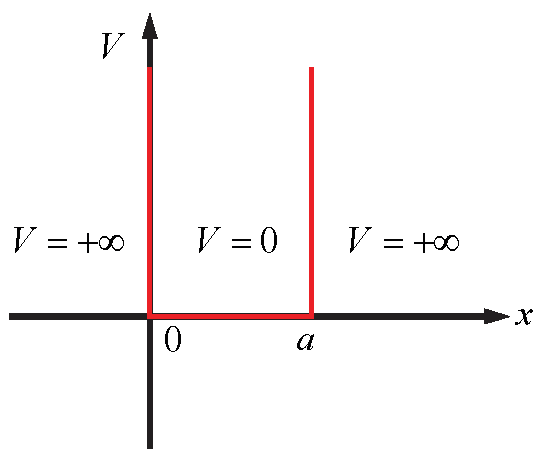
\includegraphics[width=5cm]{./figures/ISW.pdf}
\caption{无限深势阱} \label{ISW_fig1}
\end{figure}
求解定态薛定谔方程 % 链接未完成
\begin{equation}
 - \frac{\hbar ^2}{2m}\frac{d^2}{d{x^2}}\psi \left( x \right) + V\left( x \right) = E\psi \left( x \right)\text{.}
\end{equation} 
\subsection{结论} 

第 $n$ 个能级为
\begin{equation}
{E_n} = \frac{{\pi ^2}{\hbar ^2}}{2m{a^2}}{n^2} \quad (n = 1,2,3...)
\end{equation}
能量的本征波函数为
\begin{equation}
\psi \left( x \right) = \sqrt {\frac{2}{a}} \sin \left( {\frac{n\pi }{a}x} \right)
\end{equation}

\subsection{推导} 
先考虑势阱内部($0 \le x \le a$,  $V = 0$),方程变为
\begin{equation}
- \frac{\hbar ^2}{2m}\frac{{d^2}\psi \left( x \right)}{d{x^2}} = E\psi \left( x \right) 
\end{equation}
这是二阶常系数齐次微分方程.通解为
\begin{equation}
\psi \left( x \right) = {C_1}\cos \left( {kx} \right) + {C_2}\sin \left( {kx} \right) 
 k = \frac{\sqrt {2mE} }{\hbar }
\end{equation} 
其中
(通解也可以写成指数函数 $C{\E^{\I kx}}$, 加上边界条件后的结论一样)
现在讨论边界条件: 在有限深势阱束缚态中将会看到,如果势阱外部势能是有限值,波函数将会按照指数函数衰减,势能越高衰减得越快.而现在势阱外部势能为无穷大,就可以直接认为波函数在势阱外部始终为零.所以边界条件为
 \begin{equation}
\psi \left( 0 \right) = 0 \text{,}\psi \left( a \right) = 0
\end{equation}
这两个条件代入以上通解中,解得
\begin{equation}
{C_2} = 0\text{, } k = \frac{n\pi }{a} \text{.(} n = 1,2,3... \text{).}
\end{equation}

 ${C_1}$ 的取值暂时不能确定,但先将通解写为 $\psi \left( x \right) = C\sin \left( {\frac{{n\pi }}{a}x} \right)$, 常数 $C$ 就可以通过波函数的归一化%(链接未完成)
 来确定:
 \begin{equation}
1 = \int_{ - \infty }^{ + \infty } {{{\left| {\psi \left( x \right)} \right|}^2}dx}  = \int_{ - a}^{ + a} {{{\left| {C\sin \left( {\frac{n\pi }{a}x} \right)} \right|}^2}dx}  = {\left| C \right|^2}\frac{a}{2}\text{.  }
\end{equation}
严格来说, $C$ 可以是复数,解为 $C = \sqrt {{2}/{a}} {\E^{\I \theta }}$. 但是为了方便通常把归一化常数中的相位因子${\E^{\I\theta }}$ 默认为 $1$. 所以归一化的波函数为
 \begin{equation}
\psi \left( x \right) = \sqrt {\frac{2}{a}} \sin \left( {\frac{n\pi }{a}x} \right)
\end{equation}
另外,由
\begin{equation}
\frac{\sqrt {2mE} }{\hbar } = k = \frac{n\pi }{a}
\end{equation}
可以得出能级是离散的结论.即
 \begin{equation}
{E_n} = \frac{{\pi ^2}{\hbar ^2}}{2m{a^2}}{n^2} \left( {n = 1,2,3...} \right)
\end{equation}

